\documentclass[../main.tex]{subfiles}

\begin{document}
    \begin{center}
        \subsection{Методики измерений}
    \end{center}
    Основным методом исследования образцов в данной работе является \textbf{измерение 
    фотолюминисценции}. Поскольку основной задачей является получение твердотельных лазеров 
    на основе HgCdTe наногетероструктур, работающих в разумном диапазоне температур (77-300K),
    при котором возможно функционирование лазера с охлаждением жидким азотом,
    оценка зависимости интенсивности вынужденного или спонтанного излучения в зависимости от 
    температуры и внутренней структуры образцов представляет особый интерес.

    Исследуемый образец помещается в вакуумный криостат ARS-Cryotech с гелиевым охлаждением и
    возможностью нагрева образцов до необходимой температуры  в пределах $7 - 300 K$. Входное 
    отверстие как правило закрывается ZnSe окном, что позволяло заводить внутрь накачку во всем 
    требуемом диапазоне $600~nm - 15~\mu m$. На выходе же стояло окно из KRS-5, которое прозрачно
    в диапазоне $600~nm-50~\mu m$.
    
    Структуры облучались лазерами с длинами волн \ra ... с мощностями \ra ... соответственно.
    При этом лазеры были импульсными или искуственно модулировались механическим способом.

    При этом использовался фурье спектрометр Bruker Vertex V80, в режиме пошагового сканирования. 
    Этот режим позволяет передвигать зеркало спектрометра дискретно, что позволяет более точно его
    позиционировать тем самым повышая эффективное разрешение и снижая коэффициент сигнал/шум.
    Кроме того в силу устройства установки зеркало может колебаться некоторое время после установки
    размывая картину, воизбежание этого съём сигнала происходил через некоторое время после 
    позиционирования.

    В качестве приемника использовался болометр производства IRLabs с 
    высокой чувствительностью в диапазоне \ra ... . Также некоторые измерения были произведены при помощи 
    полупроводникового детектора на основе MCT (также производства IRLabs), позволяющего  улавливать 
    излучение в диапазоне $\hdots - 16\~\mu m$.

    Воизбежание паразитной засветки детекторов излучением накачки (интенсивность которого на много порядков 
    превышало излучение как исследуемого спонтанного, так и вынужденного излучения образцов) использовался набор интерференционных и 
    \ra ... фильтров, позволяющий эффективно ослаблять излучение в неинтересующем нас диапазоне.

    Для снижения влияния ЭМ наводок, а также для эффективного усиления использовались 
    усилители напряжения Standford SR560, включающие в себя регулируемые частотные фильтры 6db, 12db. 
    Правильная настройка таких фильтров позволяет существенно повысить соотношение сигнал/шум, 
    а также полностью нейтрализовать гармоники 50 Hz, которые являются основной компонентой наведённого шума.

    В случае импульсного режима накачки использовался синхродетектор Standford SR850, его использование
    позволяет существенно снизить время измерения за счет отсутствия необходимости программного усреднения 
    результатов измерения встроенного АЦП. Кроме того

    Основным ПО при обработке спектров являлся Opus 7.0. В частности это позволяет записывать временно-разрещённые спектры,
    а также в существенной мере отфильтровать шумы посредством правильной рбработки интерферограммы.

    Иной важной техникой является \textbf{измерение фотопроводимости}. Этот метод позволяет с высокой степенью точности
    определять ширину запрещённой зоны полупроводниках, а также уровни размерного квантования в случае гетероструктур
    с квантовыми ямами. Это требуется для оценки содержания кадмия в барьерах и внутреннем пространстве квантовых ям, а также
    для проверки точности исполнения гетероструктуры в поперечном плоскости образца направлении.

    Фурье спектрометр в данном случае работает в режиме непрерывного сканирования, а образец охлаждается иммерсивно.
    Для таких ихмерений важно исключить влияние спектра поглощения хладагента на результирующий спектр, для этого
    минимизируется расстояние от образца до фильтров, после которого в погружном устройстве следует вакуум.
    
    Также требуется отметить, что в таком режиме измерений в силу конструктивных причин невозможно использовать вакуумированный
    крисотат с возможностью плавной регулировки температуры, ввиду этого доступно всего лишь три варианта измерений:
    при комнатной температуре 300 K, при температуре кипения жидкого азота 77K и при температуре кипения жидкого гелия 8K. В
    данной технике измерений мы можем рассматривать образец, как своего рода приемник сигнала. 
    
    Ввиду технической сложности для присоединения контактов иными способами в экспериментах использовалась простая пайка
    с индиевым припоем (выбор обусловлен схожим с образцами коэффициентом линейного температурного расширения, что позволяет 
    обеспечить надежный контакт с поверхностью полупроводника при любой температуре).

    В качестве эталонного источника излучения в данном типе измерений использовался глобар - источник излучения среднего 
    инфракрасного излучения, имеюющий спектр, близкий к спектру абсолютно чёрного тела. Такая спектральная характеристика
    позволяет проводить точную нормировку сигнала с учетом сравнения ее с заведомой известной аппаратной
    функцией прибора.
    
    Кроме вышеперечисленного оборудования использовался токовый усилитель Standford SR570, который также способен выдавать
    ток смещения. В силу специфики образцов мы можем считать их сопротивление линейным, посему полученный
    в результате измерений, сигнал не нуждается в дополнительной обработке.

\begin{figure}[h]
    \begin{minipage}[h]{\linewidth}
    \centering
    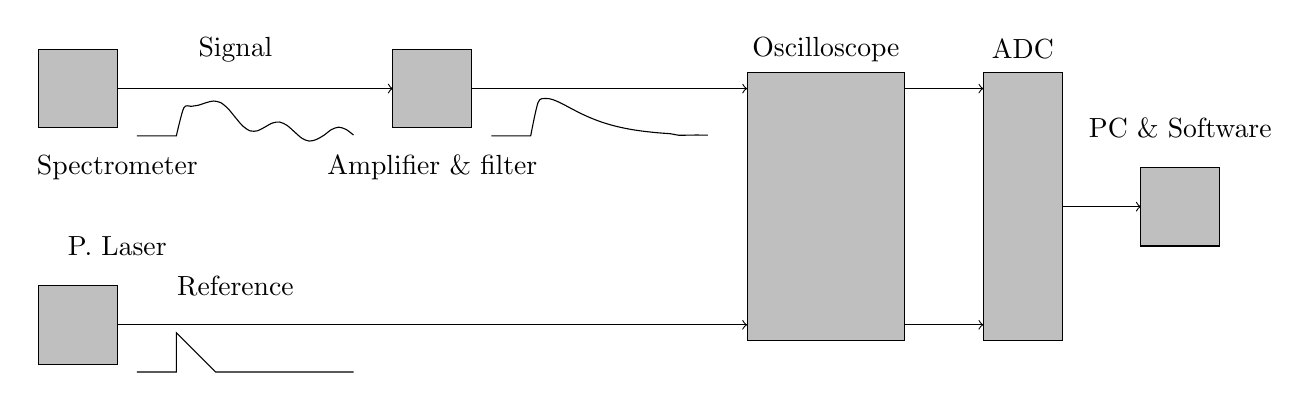
\begin{tikzpicture}
        \filldraw[fill=lightgray] (0, -2) rectangle (1, -1);
        \draw[->] (1, -1.5) -- (9, -1.5);
        \node at (2.5, -1) {Reference};
        \node at (1, -0.5) {P. Laser};
        \draw (1.25, -2.1) -- (1.75, -2.1) -- (1.75, -1.6) -- (2.25, -2.1) -- (4., -2.1);
        
        \filldraw[fill=lightgray] (0, 1) rectangle (1, 2);
        \draw[->] (1, 1.5) -- (4.5, 1.5);
        \node at (2.5, 2) {Signal};
        \node at (1, 0.5) {Spectrometer};
        \draw[domain=0:2.25] (1.25, 0.9) --
            plot[smooth] ({\x + 1.75}, {1.75 * sqrt(\x * exp(-5 * \x)) + 0.9 + 0.1 * cos(90 - 360 * 20 * \x)});
        
        \filldraw[fill=lightgray] (4.5, 1) rectangle (5.5, 2);
        \node at (5, 0.5) {Amplifier \& filter};
        \draw[->] (5.5, 1.5) -- (9, 1.5);
        \draw[domain=0:2.25] (5.75, 0.9) --
            plot[smooth] ({\x + 6.25}, {1.75 * sqrt(\x * exp(-5 * \x)) + 0.9});
            
        \filldraw[fill=lightgray] (9, -1.7) rectangle (11, 1.7);
        \node at (10, 2) {Oscilloscope};
        
        \draw[->] (11, 1.5) -- (12, 1.5);
        \draw[->] (11, -1.5) -- (12, -1.5);
        \filldraw[fill=lightgray] (12, -1.7) rectangle (13, 1.7);
        \node at (12.5, 2) {ADC};
        
        \draw[->] (13, 0) -- (14, 0);
        \filldraw[fill=lightgray] (14, -0.5) rectangle (15, 0.5);
        \node at (14.5, 1) {PC \& Software};
    \end{tikzpicture}
    \caption{\label{PLScheme} Схема измерения фотолюминисценции}
    \end{minipage}
    \vfill
    \begin{minipage}[h]{\linewidth}
        \centering
        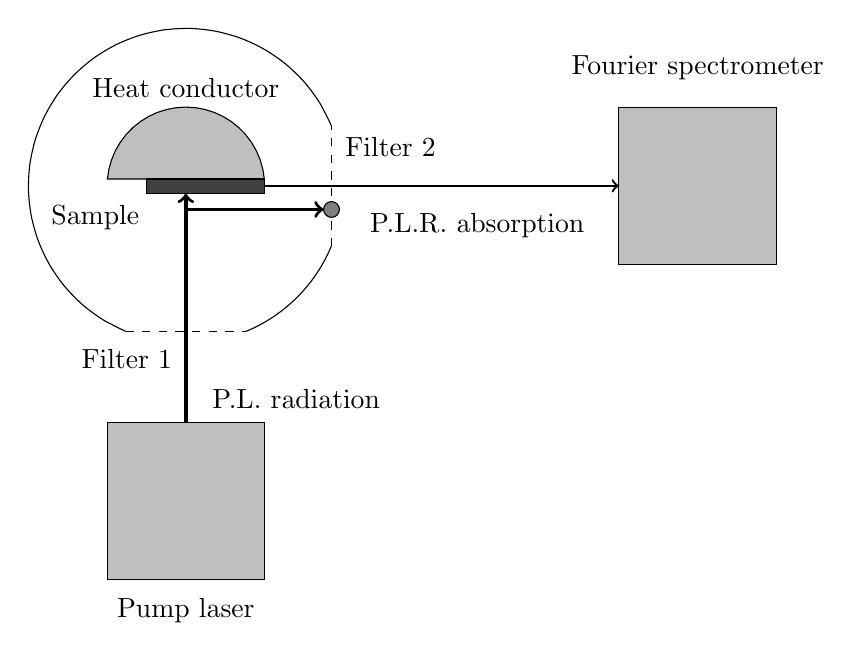
\begin{tikzpicture}
        \draw[domain=22.5:247.5] plot[smooth] ({cos(\x) * 2}, {sin(\x) * 2});
        \draw[domain=292.5:337.5] plot[smooth] ({cos(\x) * 2}, {sin(\x) * 2});
        
        \draw[dashed] ({2 * cos(247.5)}, {2 * sin(247.5)}) -- ({2 * cos(292.5)}, {2 * sin(292.5)});
        \node at (-0.75, -2.2) {Filter 1};
        
        \draw[dashed] ({2 * cos(337.5)}, {2 * sin(337.5)}) -- ({2 * cos(22.5)}, {2 * sin(22.5)});
        \node at (2.6, 0.5) {Filter 2};
        
        \filldraw[fill=lightgray, domain=5:175] plot ({cos(\x)}, {sin(\x)})
            -- ({cos(5)}, {sin(5)});
        \node at (0, 1.25) {Heat conductor};
        
        \filldraw[fill=darkgray] (-0.5, -0.1) rectangle (1., {sin(5)});
        \node at (-1.15, -0.4) {Sample};
            
        \filldraw[fill=lightgray] (-1, -5) rectangle (1., -3);
        \node at (0, -5.4) {Pump laser};
            
        \draw[->, very thick] (0, -3) -- (0, -0.1);
        \draw[->, very thick] (0, -0.3) -- (1.75, -0.3);
        \node at (1.4, -2.7) {P.L. radiation};
        \draw[fill=gray] (1.85, -0.3) circle (0.1);
        \node at (3.7, -0.5) {P.L.R. absorption};
        
        \draw[->, thick] (1, 0) -- (5.5, 0);
        
        \filldraw[fill=lightgray] (5.5, -1) rectangle (7.5, 1);
        \node at (6.5, 1.5) {Fourier spectrometer};
        \end{tikzpicture}
        \caption{\label{PLGeometry} Геометрия задачи исследования фотолюминисценции}
    \end{minipage}
    \vfill
    \begin{minipage}[h]{\linewidth}
        \centering
			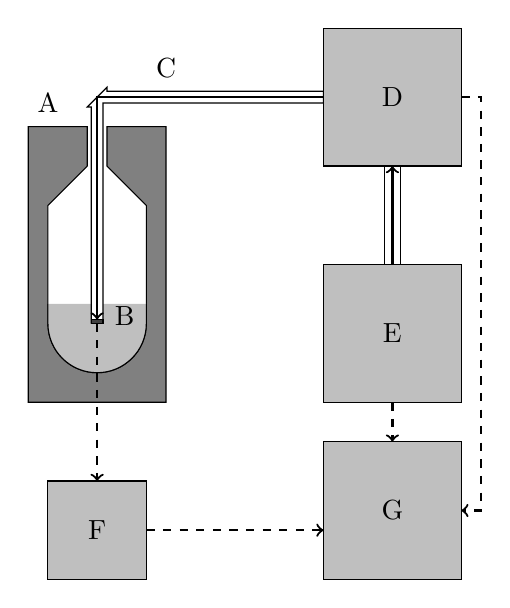
\begin{tikzpicture}
				\filldraw[fill=gray] (2,0) -- (1.5, -0.5) -- (1.5, -2)
					-- (1.5, -2) arc(0:180:-0.625)
					-- (2.75, -2) -- (2.75, -0.5) -- (2.25, 0)
					-- (2.25, 0.5) -- (3, 0.5) -- (3, -3)
					-- (1.25, -3) -- (1.25, 0.5) -- (2, 0.5) -- (2, 0);
				
				\node at (1.5, 0.8) {A};
					
				\filldraw[fill=lightgray] (1.5, -1.75)
					-- (1.5, -2) arc(0:180:-0.625)
					-- (2.75, -1.75);
					
				\node at (2.475, -1.9) {B};
					
				
				\filldraw[fill=white] (2.05, -2) -- (2.05, 0.75) -- (2, 0.75)
					-- (2.25, 1) -- (2.25, 0.95) -- (5, 0.95)
					-- (5, 0.8) -- (2.2, 0.8) -- (2.2, 0.75)
					-- (2.2, -2);
					
				\node at (3, 1.25) {C};
					
				\filldraw[fill=darkgray] (2.05, -2) rectangle (2.2, -1.95);
				
				\draw[->, thick, dashed] (2.125, -2) -- (2.125, -4);
				
				\draw[->, thick] (5, 0.875) -- (2.125, 0.875) -- (2.125, -1.95);
				
				\filldraw[fill=lightgray] (1.5, -5.25) rectangle (2.75, -4);
				
				\node at (2.125, -4.625) {F};
				
				\filldraw[fill=lightgray] (5, 0) rectangle (6.75, 1.75);
				
				\node at (5.875, 0.875) {D};
				
				\filldraw[fill=lightgray] (5, -3) rectangle (6.75, -1.25);
				
				\node at (5.875, -2.125) {E};
				
				\draw (5.775, -1.25) rectangle (5.975, 0);
				
				\draw[->, thick] (5.875, -1.25) -- (5.875, 0);
				
				\filldraw[fill=lightgray] (5, -5.25) rectangle (6.75, -3.5);
				
				\node at (5.875, -4.375) {G};
				
				\draw[->, thick, dashed] (5.875, -3) -- (5.875, -3.5);
				
				\draw[->, thick, dashed] (2.75, -4.625) -- (5, -4.625);
				
				\draw[->, thick, dashed] (6.75, 0.875) -- (7, 0.875)
					-- (7, -4.375) -- (6.75, -4.375);
            \end{tikzpicture}
            \caption{\label{PCScheme} Принципиальная схема измерения фотопроводимости}
            A - сосуд Дюара, B - жидкий гелий или азот, C - оптический тракт, D - фурье-спектрометр, 
            E - источник излучения, G - ПК и ПО.
    \end{minipage}
\end{figure}


    В ходе работы были проведено множество экспериментов по измерению фотлюминисценции образцов.
    Однако для иллюстрации зависимости порога Оже-процесса и температуры гашения СИ были избранны 
    два образца:

    Первым примером будет образец из ещё не вышедше статьи \cite{Utochkin}. Рассматривался образец, содержащий 10 несвязанных
    (имеющих меж собой широкие и "высокие" барьеры) квантовых ям
    состава Hg${}_{0.903}$Cd${}_{0.097}$Te/Cd${}_0.7$Hg${}_{0.3}$Te и толщиной 7.4 $nm$, что соответствует ширине 
    запрещённой зоны около 90 $meV$ ($\lambda \sim 14~\mu m$) при $T = 18 ~K$. Структура не была намеренно легирована; остаточная концентрация 
    носителей p-типа, полученная на основе холловских измерений, составляла порядка единиц $10^10~cm^{-2}$, а типичная 
    плотность дислокаций $\sim 10^6~cm^{-2}$. Дизайн структуры ориентирован на эффективную локализацию света вблизи КЯ, для 
    чего массив КЯ был выращен в волноводном слое толщиной в единицы мкм. Выбранное направление роста (013) 
    препятствует использованию сколотых граней кристалла в качестве зеркал резонатора, т.к. плоскости сколов образуют
    острый угол с плоскостью КЯ.

    Второй образец использовался в статье \cite{Fadeev} и представляет собой 10 КЯ состава Cd0.1Hg0.9Te/Cd0.65Hg0.35Te.
    Этот образец имеет ширину запрещённой зоны порядка 70 $meV$ ($\lambda \sim 18~\mu m$) и позволяет наблюдать стимулированное 
    излучение на этой длине волны в диапазоне  20-40 K. В остальном эта структура аналогична предыдущей.

    В ходе измерения были получены следующие спектры сфотолюминисценции:

    [спектры]

    Как можно видеть, при изменении температуры происходит сдвиг излучения в сболее коротковолновую область, а также снижение 
    интенсивности стимулированного излучения. Отчасти снижение структуры может быть объсянено тем, что длина волны становится 
    нерезонансной для внутренней волноводной структуры. С другой стороны, за счет нетипичного поведения ширины запрещенной 
    зоны от температуры (для большинства иных материалов ширина запрещённой зоны падает с ростом температуры) начинается излучение
    с меньшей длиной волны, что не так пагубно сказывается на добротности волновода как её рост. Отсюда можно сделать вывод о том, 
    что этот эффект в данном случае не так существенен. Куда больше интереса представляет сравнение времен излучательной и 
    Оже-рекомбинации, yесмотря на то, что с ростом ширины запрещенной зоны темп излучательных процессов в целом возрастает, 
    как и порог безызлучательных процессов. Также возрастает населенность состояний с более высокой энергией, что напротив ё
    стимулирует Оже-рекомбинацию.

    Отсюда возникает задача сравнения порога Оже-рекомбинации и тепловой энергии частиц.
    \newpage
\end{document}